\runningheader{Oppgave e) (frivillig)}{}{Side \thepage\ av \numpages}

% ********************************************************
% oppgave e) 
% ********************************************************  
\item
  Lag følgende modell hvor den nye blokken er {\it  Derivative}. 
  \begin{figure}[H]
    \centering
    \hspace*{0mm}\scalebox{0.78}{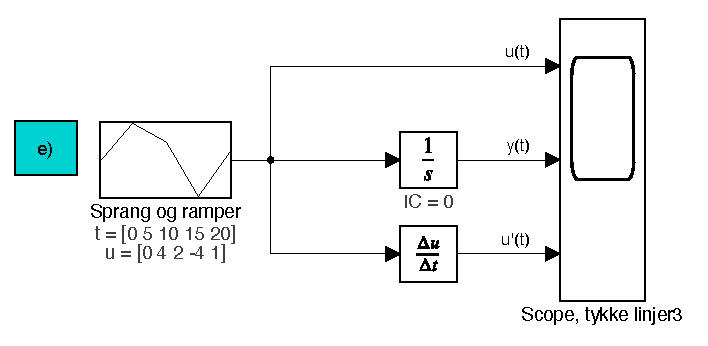
\includegraphics{2e.pdf}}
  \end{figure}
  Signalet $u(t)$ er modellert med {\sf Sprang og ramper}-blokken
  med følgende verdier
  \begin{itemize}
  \item   {\sf Tidspunkter} som {\tt [0~5~10~15~20]}
    \item {\sf Utgangsverdier} som {\tt [0~4~2~-4~1]} 
  \end{itemize}
  og med interpolasjonsmetode som \dbox{\sf Linear} fra
    rullegardinmenyen i blokken.  
  {\color{red}La simuleringstiden fortsatt være 25 sekund.}

    {\bf Gjør følgende oppgaver / svar på følgende spørsmål:    }
  
  \begin{enumerate}[label=e\arabic*)]
    \setlength\itemsep{0mm}
    \item   Simuler modellen og ta med simuleringsresulatet
    i innleveringen din. 
  \item Beregn arealet under $u(t)$ (ta hensyn til både positiv og
    negativt areal).
  \item Hvordan henger dette arealet sammen responsen i $y(t)$?
  \item Hva viser resultatet for den deriverte $u'(t)$? 
    Forklar sammenhengen mellom $u(t)$ og $u'(t)$.
  \end{enumerate}
   
